\documentclass[a4paper, 11pt]{article}
\usepackage{comment} % enables the use of multi-line comments (\ifx \fi) 
\usepackage{lipsum} %This package just generates Lorem Ipsum filler text. 
\usepackage{fullpage} % changes the margin
\usepackage{graphicx}

\usepackage[
singlelinecheck=false % <-- important
]{caption}

\begin{document}
%Header-Make sure you update this information!!!!
\noindent
\large\textbf{Homework 4} \hfill \textbf{Group 18} \\
\normalsize Department of Information Engineering \hfill Aladdine Ayadi\\
Big Data Computing \hfill Giovanni Barbieri\\
Prof. Andrea Pietracaprina \hfill Alessandro Pelizzo\\
Due Date: 31/05/2018 \hfill Davide Talon


\section*{Test results}
In the present report the times needed for the construction of the coreset, the running time of the sequential algorithm and the load time of different datasets are analyzed.
Let $N_{exec}$ be the number of cores per executor for a total number of $N_{tot}$  cores used. The measurements evaluate the time $t_c$ which denotes the time for the construction of the coreset, $t_s$ represents the time for the run of sequential algorithm and finally $t_l$ the time needed for the loading and count of points in the dataset.
Figure \ref{image:a} shows that the heaviest operations of the algorithm are the loading of the dataset and the construction of the coreset,  while the time needed by the sequential algorithm for the construction of the final centers is proportional to the number of partitions, this is probably due to the cost of communication among different partitions.
Incresing the number of centers greater times are noticed  in terms of $t_c$ and $t_s$ while the time for the loading of the dataset is steady. As expected the average distance among points deacreases with the number of centers, as shown in Figure \ref{image:b}.
Different times for the same simulation settings lead us to conjecture that the load of the cluster influences the performance obtained.


\bgroup
\vspace{0pt}
\def\arraystretch{0.9}%  1 is the default, change whatever you need
\begin{footnotesize}
	\begin{table}[!htb]
		\centering
		\vspace{10pt}
		\parbox[t]{.45\linewidth}{
		\begin{tabular}{c|c|c|c|c} 
			\hline
			\textbf{$N_{tot}$} & \textbf{$N_{exec}$} & \textbf{$t_c [ms]$} & \textbf{$t_s [ms]$} & \textbf{$t_l [ms]$} \\
			\hline
			4 & 2 & 14785 & 165 & 169256\\ 
			8 & 2 & 7262 & 194 & 92361 \\
			8 & 4 & 12393 & 174 & 114576\\
			8 & 8 & 23183 & 324 & 229915\\
			16 & 4 & 22651 & 229 & 147105\\
			16 & 8 & 22902 & 212 & 215455\\
			32 & 4 & 14832 & 256 & 257419\\
			32 & 8 & 24426 & 516 & 227701\\
			64 & 4 & 19192 & 299 & 148242\\
			64 & 8 & 22688& 188 & 206375\\
			\hline
		\end{tabular}
		\caption{Results with dataset \textit{all}, $P=32$, $k=20$  and increasing cores.}\label{table:a}
		}
	\end{table}
\end{footnotesize}
\egroup
\bgroup
\vspace{0pt}
\def\arraystretch{0.9}%  1 is the default, change whatever you need
\begin{footnotesize}
\begin{table}[!htb]	
\parbox[t]{.45\linewidth}{
\centering
		\vspace{0pt}
		\begin{tabular}[htb]{c|c|c|c} 
			\hline
			\textbf{$P$} & \textbf{$t_c [ms]$} & \textbf{$t_s [ms]$} & \textbf{$t_l [ms]$} \\
			\hline
			4 &  12402 &  21 & 346732\\ 
			8 & 7808 &  36  & 42784\\
			16 &  4885 &  80 & 40415\\
			32 & 3037 &  195 & 33901\\
			64 &  9715&  607& 44835\\
			128 &  4139 & 2050 & 43149\\
			256 & 5222 &  8189 & 38288 \\
			\hline			
		\end{tabular}
		\vspace{10pt}
	%\caption{Results with dataset \textit{all}, $N_{tot} = 32$, $N_{exec} = 4$, $k=20$  and increasing $P$.}\label{table:b}
}
		\hfill	
\parbox[t]{.45\linewidth}{
		\centering
		\vspace{0pt}
		\begin{tabular}[htb]{l|c|c|c} 
			\hline
			\textbf{Dataset} & \textbf{$t_c [ms]$} & \textbf{$t_s [ms]$} & \textbf{$t_l [ms]$} \\
			\hline
			vectors-50-500000 &  1848 &  170 & 26885\\
			vectors-50-1000000 &  2190  &  193  & 31254 \\ 
			vectors-50-2000000 &  5325&    179& 73585\\
			vectors-50-3000000&  2486 &  232 &40012 \\
			vectors-50-all &  3037 &  195 & 33901\\
			\hline
		\end{tabular}
%		\vspace{10pt}
%		\caption{Results with dataset \textit{all}, $N_{tot} = 32$, $N_{exec} = 4$, $k=20$  and increasing $P$.}\label{table:b}
}
\hfill
\parbox[t]{.45\linewidth}{
		\caption{Results with dataset \textit{all}, $N_{tot} = 32$, $N_{exec} = 4$, $k=20$  and increasing $P$.}\label{table:b}
		}
				\hfill	
\parbox[t]{.45\linewidth}{
		\caption{Results with $N_{tot} = 32$, $N_{exec} = 4$, $k=20$, constant number of partitions $P$  and increasing size of the dataset.}\label{table:c}
			}
	\end{table}
\end{footnotesize}
\egroup
\begin{figure}
	\vspace{0pt}
  \centering
      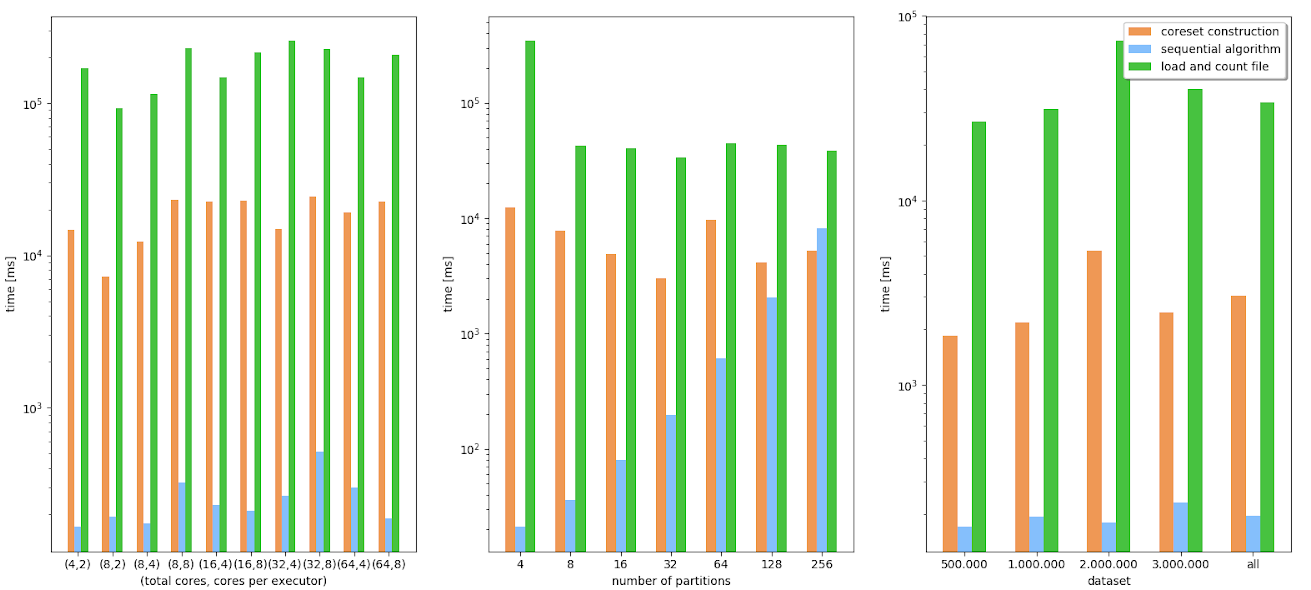
\includegraphics[scale=0.35]{grafici.png}
  \caption{Results of the different simulations respectively with increasing cores, partitions and dataset size, times are represented in a logaritmic scale.}\label{image:a}

\end{figure}

\begin{figure}

  \centering
      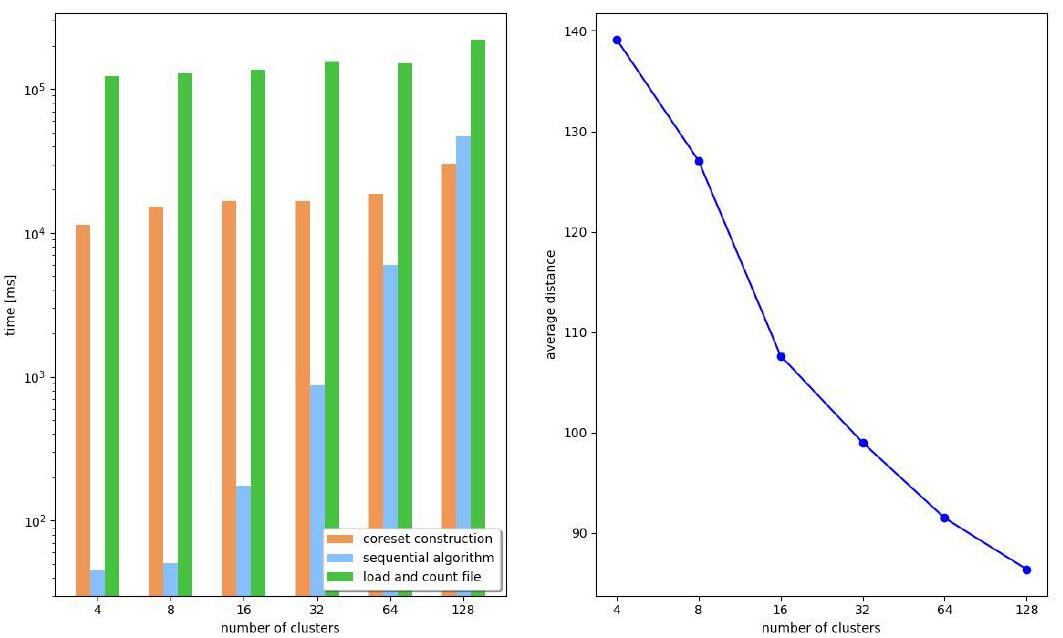
\includegraphics[scale=0.35]{result.jpg}
  \caption{Results for the simulations with increasing number of centers with $N_{tot} = 32$, $N_{exec} = 4$ and $P=32$. The image on the left represents the performances in terms of times expressed in a logaritmic scale, while the one on the right shows the average distance, i.e.the sum of centers pairwise distances divided their number.}\label{image:b}
\end{figure}




\end{document}
